\documentclass{standalone}

\usepackage{tikz}
\usetikzlibrary{shapes}
\usetikzlibrary{arrows}
\usetikzlibrary{positioning}
\usetikzlibrary{calc}
\usetikzlibrary{fit}
\begin{document}
    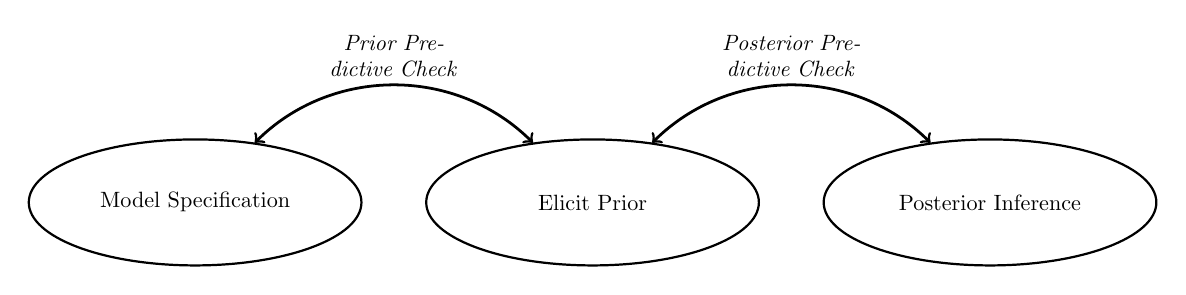
\begin{tikzpicture}[
        scale=0.8,
        transform shape, thick,
        every node/.style={text width=3.5cm, align=center},
        constructs/.style = {draw,
                            ellipse,
                            minimum width=4cm,
                            minimum height=2cm}
        ]
        \node[constructs] (Model) {Model Specification};
        \node[constructs] [right = of Model] (Prior) {Elicit Prior};
        \node[constructs] [right = of Prior] (Posterior) {Posterior Inference};
        \draw [<->, line width=1pt] (Model) to [out=45,in=135] node[above] {\textit{Prior Predictive Check}} (Prior);
        %\draw [->, line width=1pt] (Priori) to [out=225,in=315] {} (Modelo);
        \draw [<->, line width=1pt] (Prior) to [out=45,in=135] node[above] {\textit{Posterior Predictive Check}} (Posterior);
        %\draw [->, line width=1pt] (Posterior) to [out=225,in=315] {} (Priori);
    \end{tikzpicture}
\end{document}
